\documentclass[tikz,border=10pt]{standalone}
\usepackage{pgfplots}
\usetikzlibrary{calc}

\begin{document}

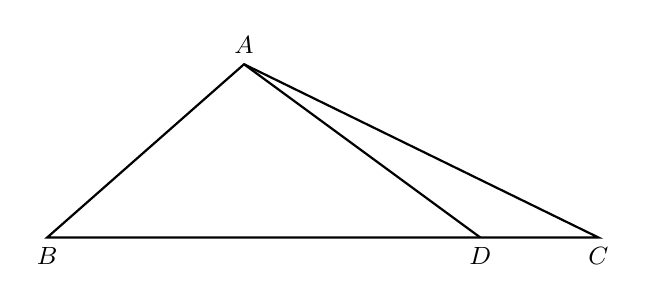
\begin{tikzpicture}[>=stealth, thick, font=\small]
    % 1. 定义顶点坐标 (根据图像比例估算)
    % 设定 B 为原点，C 在 x 轴上
    \coordinate (B) at (0,0);
    \coordinate (C) at (7,0);
    \coordinate (A) at (2.5,2.2);
    \coordinate (D) at (5.5,0); % D 在 BC 边上靠近 C 的位置

    % 2. 绘制主要三角形边界
    \draw (A) -- (B) -- (C) -- cycle;

    % 3. 绘制内部连线 AD
    \draw (A) -- (D);

    % 4. 标注顶点字母
    % 使用 anchor 确保字母不在线条上，且位置与原图一致
    \node[above] at (A) {$A$};
    \node[below] at (B) {$B$};
    \node[below] at (C) {$C$};
    \node[below] at (D) {$D$};

    % (可选) 如果需要强调 D 点，可以画一个小圆点
    % \fill (D) circle (1.5pt);

\end{tikzpicture}

\end{document}